\section{Proposal}
\label{sec:Proposal}

This Section wraps up the previous considerations by making a partial proposal
for the missing elements, so that it becomes possible to demonstrate that our vision
works. We demonstrate that it becomes possible to specify MAs independently of the
MT specifying a \DSL's execution semantics; that several MAs may be linked to
the same MT for animating a model according to the viewer's preferences; and finally
that MAs may be reused accross \DSLs.

%We start by specifying a prototype metamodel \textsf{CS} for specifying concrete
%syntaxes explicitly. We then define 

\subsection{\textsf{VCS}: The Visual Concrete Syntax \DSL}
\label{sec:Proposal-VCS}

\autoref{fig:VCS} shows the metamodel of a \textsf{VCS}, a simplified \DSL designed
for the specification of Visual Concrete Syntaxes. It consists of a \textsf{Canva}
of variable size where graphical elments (\textsf{GElement}) may be geometrically
placed. A \textsf{GElement} follows the Composite Pattern \citep{B:Gamma-etAl:1995}:
\textsf{Shape}s may be \emph{composed}, i.e. the \textsf{containee} is displayed
\emph{inside} the \textsf{container} with specific alignment features. 

A \textsf{Shape} is either a \textsf{Table}, a \textsf{TextBox}, or a 
\textsf{Geometric} element, which is either a \textsf{Form} or a 
\textsf{Connector}. Each \textsf{Shape} is inscribed into a bouding box with specific 
dimensions that helps precisely positioning it on the \textsf{Canva}, and also
defines specific features: for example, a Rectangle may define the thickness of its
external box, and an Arrow may define different types and sizes for their heads.
A \textsf{Shape} may also define a \textsf{Style} that can be \textsf{name}d and
reused for other \textsf{Shape}s, to specify various features such as the background
or line colour, the line transparency, etc.

This metamodel captures insideness with \textsf{Composer}, and may easily be extended
with additional \textsf{Shape}s that only need to be encapsulated in a box (thus,
giving value to the attributes \textsf{length} and \textsf{height} in \textsf{Shape}).


\begin{figure}[t]%
   \centering
   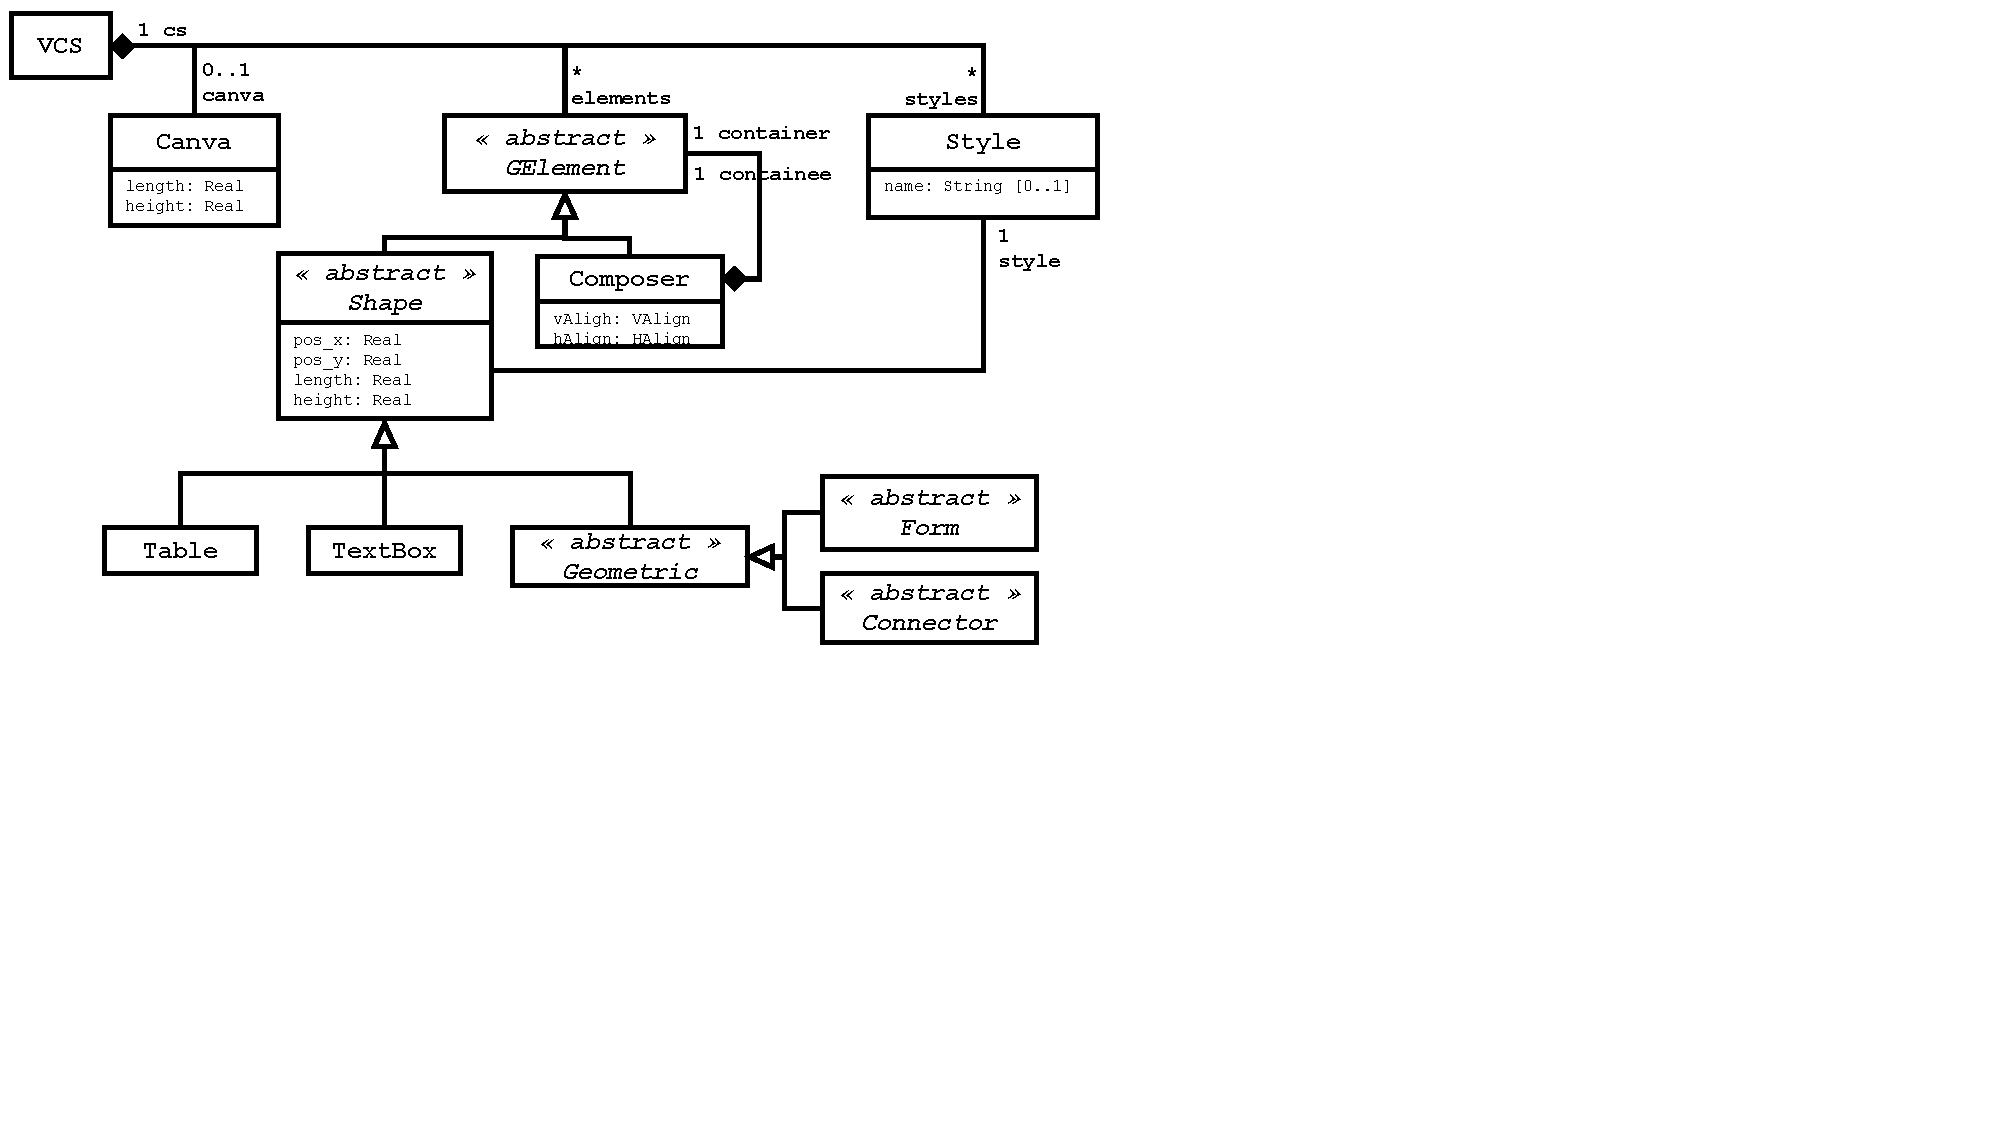
\includegraphics[width=\columnwidth,clip, trim=0cm 9cm 15cm 0.2cm]{VCS}%
   \caption{\textsf{VCS}: A simplified \DSL for specifying \emph{V}isual \emph{C}oncrete \emph{S}yntaxes}%
   \label{fig:VCS}%
\end{figure}


\subsection{Revisiting the \textsf{FSM}}
\label{sec:Proposal-FSM-CS}

We now informally define a mapping from the \DSL specifying the abstract syntax 
of the \FSM \DSL, as presented in \autoref{fig:FSM_MM}, with the elements of 
\textsf{VCS}. 

The \textsf{FSM} itself is simply mapped to the general \textsf{Canva}, but we put
a \textsf{TextBox} on the top left that will display the value of \textsf{FSM::name}.
A \textsf{State} will be represented by an \textsf{Ellipse} with equal \textsf{length}
and \textsf{height} (thus forming a circle) drawn in black. A final \textsf{State}
is simply the composite of two \textsf{Ellipse}s vertically and horizontally centered,
whose dimensions only differ by a specific delta. For the purpose of simplification,
we will represent initial states with a similar \textsf{Ellipse} using a dotted line.
A \textsf{Transition} will be represented by a \textsf{Curved} \textsf{Connector}
using a black, plain line, with the same thickness as the \textsf{Ellipse}s, and
with an \textsf{Arrow} of the biggest size on the end part. 

Following the traditional approach in \MDE, this mapping should generate a so-called
\emph{palette} that allows modellers to create their models. From this simple example,
we see that such a definition should introduce flexibility for the modeller. 
For example, the \textsf{Transition} may require different types of \textsf{Connector}s
depending on the model's complexity.
